
%(BEGIN_QUESTION)
% Copyright 2013, Tony R. Kuphaldt, released under the Creative Commons Attribution License (v 1.0)
% This means you may do almost anything with this work of mine, so long as you give me proper credit

Karbondioksidgass (CO$_{2}$) absorberer visse frekvenser av infrarødt lys svært godt. Med dette som bakgrunn forsøkte jeg en gang å bygge min egen CO$_{2}$-gassanalysator med følgende oppsett:

$$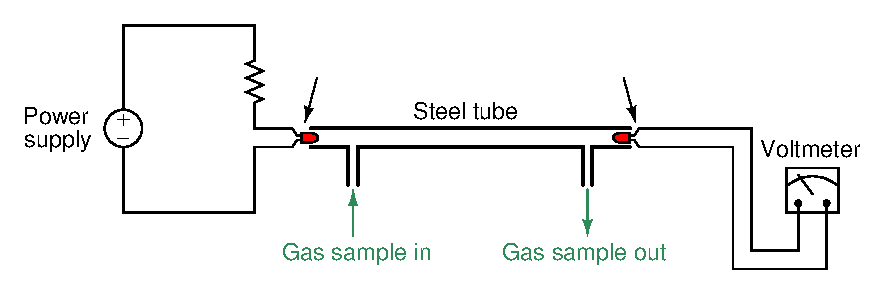
\includegraphics[width=15.5cm]{i00563x01.eps}$$

Ved testing av oppsettet mot tre kjente CO$_{2}$-kilder målte jeg svært uventede resultater:

% No blank lines allowed between lines of an \halign structure!
% I use comments (%) instead, so that TeX doesn't choke.

$$\vbox{\offinterlineskip
\halign{\strut
\vrule \quad\hfil # \ \hfil & 
\vrule \quad\hfil # \ \hfil & 
\vrule \quad\hfil # \ \hfil \vrule \cr
\noalign{\hrule}
%
% First row
{\bf Gasskilde} & {\bf CO$_{2}$-innhold} & {\bf Fotodiode-utgangsspenning} \cr
%
\noalign{\hrule}
%
% Another row
Omgivelsesluft & Lavt & Moderat \cr
%
\noalign{\hrule}
%
% Another row
Utåndingsluft & Moderat & Lav \cr
%
\noalign{\hrule}
%
% Another row
Ren CO$_{2}$ & Høyt & Høy \cr
%
\noalign{\hrule}
} % End of \halign 
}$$ % End of \vbox

Omgivelsesluften kom fra en trykkluftlinje i et verksted. Kilden for ren CO$_{2}$ var en høytrykksflaske med CO$_{2}$ brukt til MIG-sveising.

\vskip 10pt

Angi hvordan fotodiodespenningen {\it burde} ha reagert dersom oppsettet faktisk målte CO$_{2}$-innhold. Lag deretter en hypotese om hva oppsettet {\it faktisk} målte, hvis det ikke var CO$_{2}$.

\underbar{file i00563}
%(END_QUESTION)





%(BEGIN_ANSWER)

Slik burde responsen vært dersom det virkelig var CO$_{2}$ som ble målt:

% No blank lines allowed between lines of an \halign structure!
% I use comments (%) instead, so that TeX doesn't choke.

$$\vbox{\offinterlineskip
\halign{\strut
\vrule \quad\hfil # \ \hfil & 
\vrule \quad\hfil # \ \hfil & 
\vrule \quad\hfil # \ \hfil \vrule \cr
\noalign{\hrule}
%
% First row
{\bf Gasskilde} & {\bf CO$_{2}$-innhold} & {\bf Ideell fotodiode-utgangsspenning} \cr
%
\noalign{\hrule}
%
% Another row
Omgivelsesluft & Lavt & {\it Høy} \cr
%
\noalign{\hrule}
%
% Another row
Utåndingsluft & Moderat & {\it Moderat} \cr
%
\noalign{\hrule}
%
% Another row
Ren CO$_{2}$ & Høyt & {\it Lav} \cr
%
\noalign{\hrule}
} % End of \halign 
}$$ % End of \vbox


%(END_ANSWER)





%(BEGIN_NOTES)

Min egen hypotese er at oppsettet målte {\it vanndampkonsentrasjon} heller enn CO$_{2}$-konsentrasjon, siden vanndamp har et bredere absorpsjonsbånd i infrarødt enn karbondioksid, og vanndampinnholdet i de tre prøvekildene samsvarer bedre med måleresultatene:

% No blank lines allowed between lines of an \halign structure!
% I use comments (%) instead, so that TeX doesn't choke.

$$\vbox{\offinterlineskip
\halign{\strut
\vrule \quad\hfil # \ \hfil & 
\vrule \quad\hfil # \ \hfil & 
\vrule \quad\hfil # \ \hfil \vrule \cr
\noalign{\hrule}
%
% First row
{\bf Gasskilde} & {\bf H$_{2}$O-innhold} & {\bf Fotodiode-utgangsspenning} \cr
%
\noalign{\hrule}
%
% Another row
Omgivelsesluft & Moderat & Moderat \cr
%
\noalign{\hrule}
%
% Another row
Utåndingsluft & Høyt & Lav \cr
%
\noalign{\hrule}
%
% Another row
Ren CO$_{2}$ & Lavt & Høy \cr
%
\noalign{\hrule}
} % End of \halign 
}$$ % End of \vbox


%INDEX% Måling, analytisk: karbondioksid
%INDEX% Måling, analytisk: vanndamp i luft
%INDEX% Kjemi, spektroskopi

%(END_NOTES)

